%\documentclass[14pt]{report}
\documentclass[14pt]{../../DSTUreport/sty/DSTUReport} % Базовый стиль - поправленный стандартный report, они взаимозаменяемы

\RequirePackage{../../DSTUreport/sty/DSTUExtra} % Расширение над DSTUReport, включая longtable, caption, biblatex и прочие must have пакеты
\RequirePackage{../../DSTUreport/sty/DSTUTitles}

% Не забудьте переключить титульный лист
\RequirePackage{../../DSTUreport/sty/DSTUEskd} % Изменения стиля под ГОСТ 2.105

\sloppy

% Даты начала и конца работы
\renewcommand{\startDay}			{0}
\renewcommand{\startMonth}			{декабря}
\renewcommand{\startYear}			{2024}
\renewcommand{\finalDay}			{20}
\renewcommand{\finalMonth}  		{декабря}
\renewcommand{\finalYear}			{2024}
\renewcommand{\finalDate}			{<<\finalDay>> \finalMonth\ \finalYear г.}
% Сокращения официальных названий
\renewcommand{\schoolNameFull}		{Институт опережающих технологий <<Школа Икс>>}
\renewcommand{\schoolName}			{ДГТУ ИОТ <<Школа Икс>>}
\renewcommand{\orgNameFull}			{
	ФЕДЕРАЛЬНОЕ ГОСУДАРСТВЕННОЕ БЮДЖЕТНОЕ
	ОБРАЗОВАТЕЛЬНОЕ УЧРЕЖДЕНИЕ ВЫСШЕГО ОБРАЗОВАНИЯ
	«ДОНСКОЙ ГОСУДАРСТВЕННЫЙ ТЕХНИЧЕСКИЙ УНИВЕРСИТЕТ»
	}
\renewcommand{\orgName}				{ФГБОУ ВО <<ДГТУ>>}
% Личная информация
\renewcommand{\facKey}				{15.03.06} % номер направления подготовки
\renewcommand{\facName}				{Мехатроника и робототехника} % название направления подготовки
\renewcommand{\decim}				{\facKey.930000.000} % Для рамок, поищи в DSTUEskd.sty
\renewcommand{\developer}			{Лемешкин}
\renewcommand{\developerIOF}		{Р. А. \developer}
\renewcommand{\developerFaImOt}		{\developer Руслан Андреевич}
\renewcommand{\developerYear}		{3} % курс обучения (скорее всего ты его будешь менять чаще всего ;)
\renewcommand{\developerGroup}		{ХР\developerYear}
% Названия конкретного документа
\renewcommand{\docTypeFull}			{Отчёт по ЛР} % Тип документа (тоже в DSTUEskd.sty ищи)
\renewcommand{\docType}				{ЛР}
\renewcommand{\module}				{Информационные устройства роботов и РТС} % Вид практики или название дисциплины курсача
\renewcommand{\internOrg}			{\schoolName} % Название предприятия практики
\renewcommand{\devNameFull}			{\module} % Название темы для курсача
\renewcommand{\devName}				{УД} % наверное только для рамок
% И преподы
\renewcommand{\schTutorPos}			{к.т.н., доц.} % От уника чел для практики или владелец
\renewcommand{\schTutorIOF}			{А.Ю. Зайцев}%  модуля / наставник для курсача и рамок
\renewcommand{\baseTutorPos}		{директор} % От предприятия чел для практики
\renewcommand{\baseTutorIOF}		{П.В. Герасин} % или утвердивший для курсача (директор или ректор)
\renewcommand{\nControl}			{} % смотри в файле с рамками, мож и надо...

\DSTUHaveLRIfalse		 % Вставить лист регистрации изменений
\DSTUHaveLYfalse		% Вставить лист утверждения
\DSTUHaveESKDFrametrue   % Использовать рамку

\usepackage{pdflscape}
% \usepackage{lscape}

%\makeatletter
%\newcommand{\keepwithnext}{\@beginparpenalty 10000}
%\makeatother % Особые пакеты для этого документа
% Любимые команды
\newcommand{\Code}[1]{\textbf{#1}}


   % Особые макросы для этого документа

\begin{document}

\labMain5 % вывод титульника. Вся информация для него указана
          % в preamble.ink.tex, здесь ставится только номер.
          % Нюансы реализации можно посмотреть в sty/DSTUTitles

% Также можно использовать \Referat, как в оригинале
%\begin{abstract}

\ifDSTUHaveESKDFrame
\makeatletter
\def\@oddhead{\titleFrame}
\def\@oddfoot{}
\makeatother
\fi


\setcounter{tocdepth}{3}
\tableofcontents % вставляем оглавление
\clearpage


\ifDSTUHaveESKDFrame
\clearpage
\makeatletter
\def\@oddhead{\mainFrame}
\def\@oddfoot{}
\makeatother
\fi

%\end{abstract}

%%% Local Variables: 
%%% mode: latex
%%% TeX-master: "rpz"
%%% End: 


%\include{00-acro}

\chapter*{Введение}
\section*{title}
Данный отчёт по практике можно считать документацией к роботам Жук проекта Eurobot на конец июля 2024 года и описанием технических особенностей этих роботов.

Изначальная задача, создание прошивки для робота, сильно зависит от понимания различных особенностей устройства, поэтому создание документации является важным этапом для достижения цели.

Краткий обзор отчёта:\\
В первой части описан язык программирования (ЯП) MicroPython и среда для работы с ним;\\
Во второй приведены общие положения, касающиеся робота, рисунок-схема подключений и некоторые параметры корпуса;\\
В третьей описаны особенности использованных в роботах энкодеров и мои наработки, связанные с ними;\\
В четвёртой затронуты особенности УЗ датчиков;\\
В пятой описана работа, проделанная с гироскопом.
 %% введение

\chapter{Обзор робота}
Робот (Жук) предназначен для ознакомления студентов первого и второго курса с особенностями программирования и конструирования роботов. Он представляет собой красный пластиковый цилиндр с двумя колёсами по бокам, а также упорами спереди и сзади в виде железных шариков в пластиковых креплениях. При изучении робота стало понятно, что упорам требуется доработка: надо уменьшить их высоту, чтобы опираясь на них робот не отрывал колёса от земли. Я временно решал проблему, вытаскивая один из шариков. Впоследствии было предложено разобрать робота, и уменьшить высоту внешней части крепления, добавив шайбы на крепёжные винты.

Жук управляется микроконтроллером (МК) ESP-WROOM-32 (esp32, еспшка), изображение есть на \ref{f:lb_scheme} и в открытых источниках. Также в нём есть активная периферия:
\begin{itemize}
    \item 6 УЗ-датчиков HRC SR04;
    \item 2 электромотора с энкодерами GA25-370;
    \item 1 MPU 6050 (гироскоп)(GY-521).
\end{itemize}

Важно заметить, что её можно использовать только физически отключая не используемые в данный момент элементы, при этом использовать все периферийные устройства одновременно нельзя.

Кроме перечисленного выше, 2 ультразвуковых датчика подключены через \textbf{расширитель пинов i2c pcf8574}, моторы управляются через \textbf{драйвер L9110S}, а питание идёт от аккумуляторов через \textbf{DC-DC преобразователь HW-411}. Информацию о модели аккумуляторов предстоит найти в будущем и включить в документацию. Подробнее каждый из этих элементов будет освещён в соответствующих разделах.

Ниже, на рисунке \ref{f:lb_scheme} отражена схема подключения элементов друг к другу. Рисунок был отредактирован и актуализирован мной в процессе подготовки к дальнейшей работе. Ознакомиться с оригиналом рисунка можно на доске в миро. При работе над рисунком были использованны разнообразные инструменты, предлагаемые упомянутой электронной доской и я научился более тонко работать с соединительными линиями и местами их соединения, что поможет в будущем делать аналогичные схематические рисунки других устройств.
\pagebreak[3]

\begin{figure}[!h]
    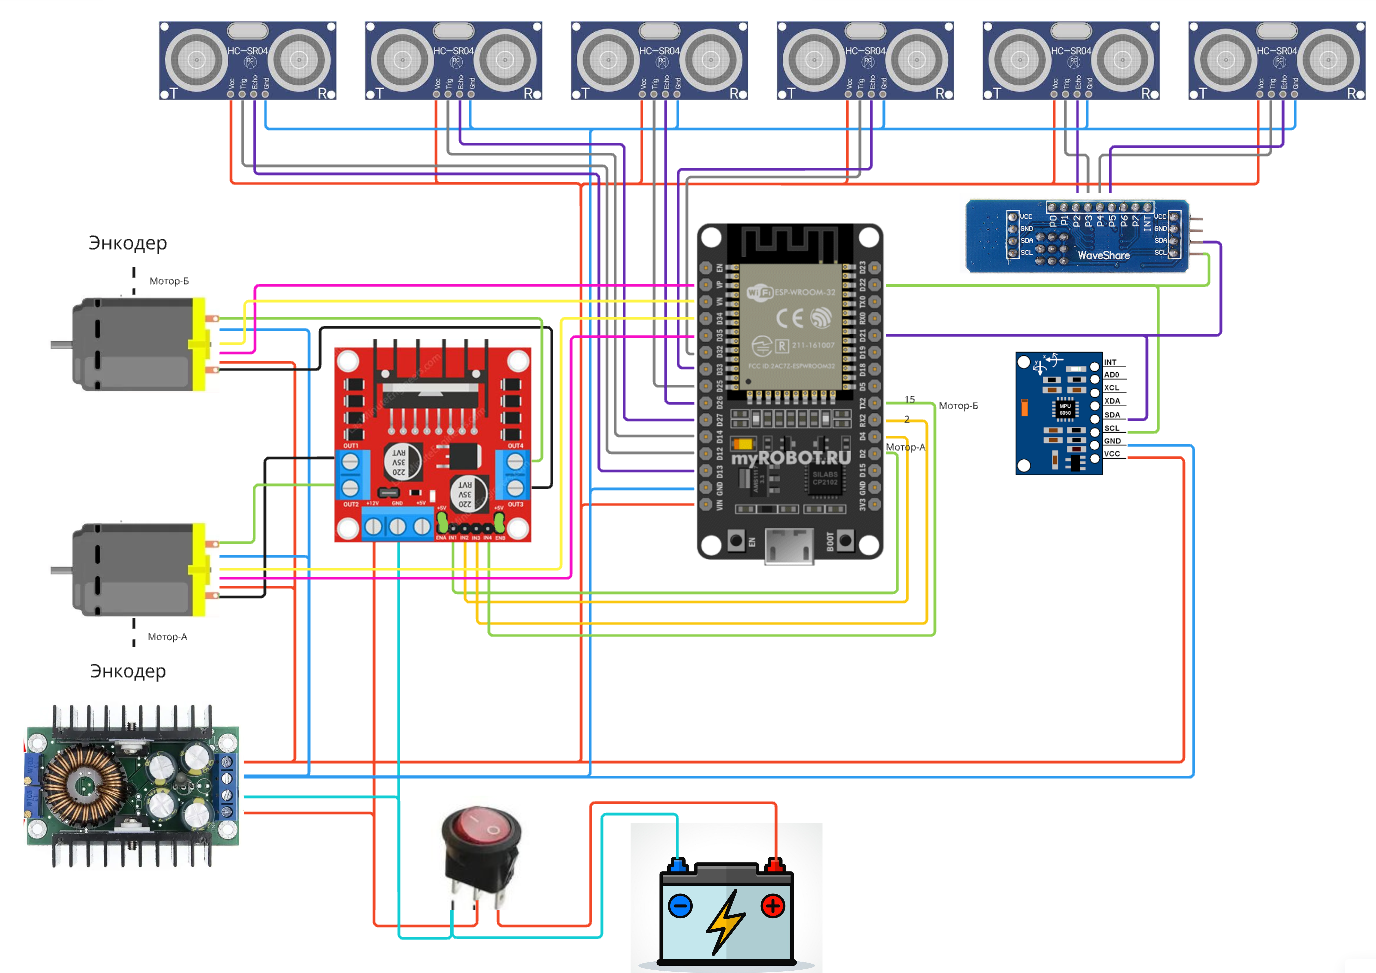
\includegraphics[width=0.95\linewidth]{./graphics/img/Ladybug_scheme.png}
    \caption{Схематический рисунок подключений}
    \label{f:lb_scheme}
\end{figure}

\pagebreak[3]
При доработке рисунка я научился:
\begin{itemize}
    \item прозванивать электрические цепи
    \item изучил сопутствующую роботу документацию
    \item выявил несоответствия реального и описанного в проекте
    \item рассмотрел чужие наработки в области создания мобильных роботов
\end{itemize}

Анализируя всё вышесказанное, можно сделать вывод, что:
\begin{enumerate}
    \item Жук обладает разнообразными датчиками для отредактирования в пространстве
    \item Жук имеет аккумуляторы для автономной работы
    \item Документация часто не соответствует действительности, и её актуализация является необходимой частью рабочего процесса
    \item При дальнейшей работе необходимо добавить к документации модель аккумуляторов
\end{enumerate}

\chapter{MicroPython}
MicroPython --- это интерпретируемый язык программирования, основанный на Python. Отличается наличием библиотек для управления микроконтроллерами и некоторыми оптимизациями для большей производительности. Был выбран по историческим причинам и из-за личных предпочтений.

Альтернативой является язык Arduino, но здесь он рассматриваться не будет, так как в моей работе не использовался.

Для правильной работы необходимо прошить МК. В рамках практики я использовал встроенные средства Thonny. При этом есть альтернативные способы, описание которых можно найти в открытых источниках.

\section{Окружение}
Для работы с кодом использовалась IDE Thonny, установленная в виртуальное окружение для Python. Создаётся виртуальное окружение последовательностью команд в терминале:

{\tt
    \noindent\hangindent=5mm\hangafter=1
    mkdir /path/to/project/directory/ \# здесь создаётся директория (папка) в котой будут храниться файлы проекта. Команда зависит от ОС (приведён пример для linux) и имеет аналоги в граф. интерфейсе

    \noindent\hangindent=5mm\hangafter=1
    cd /path/to/project/directory/ \# переход в рабочую директорию. Команда зависит от ОС (приведён пример для linux) и обязана исполняться в командой строке

    \noindent\hangindent=5mm\hangafter=1
    venv venv \# команда, которая создаёт в текущей директории папку venv и автоматически генерирует в ней необходимые файлы

}
\noindent Для активации venv надо запустить скрипт \texttt{activate}. Например:\\
\texttt{
    source /path/to/project/directory/venv/bin/activate
}\\
Сама IDE устанавливается командой \texttt{pip install thonny} внутри активированного venv.

Все библиотеки рекомендуется устанавливать локально в окружение текущего проекта, что я и сделал с помощью той же команды \texttt{pip install}.

В моём случае папкой проекта является Practice/. В ней создана папка venv, в которой собраны все автоматически генерируемые файлы. Рядом стоит создать папки для файлов с собственным кодом и файлов библиотек, либо же (для оптимизации) собрать в один файл все необходимые Функции, но при таком подходе дальнейшая разработка будет нескольно затруднена.

\section{Библиотеки}
Как было сказано ранее, важной особенностью выбранного ЯП является сильное разбиение на библиотеки, поэтому работу следует начинать как раз с выбора этих пакетов.

Для получения общей информации я задал вопрос нейросети Perplexity и она предложила мне использовать следующие библиотеки:
\begin{description}
    \item[machine] - встроенная библиотека для работы с микроконтроллером и его периферийными устройствами.\\
    Документация: https://docs.micropython.org/en/latest/library/machine.html
    \item[ustruct] - встроенная библиотека для работы с байтовыми структурами.\\
    Документация: https://docs.micropython.org/en/latest/library/ustruct.html
    \item[utime] - встроенная библиотека для работы с таймерами и датой.\\
    Документация: https://docs.micropython.org/en/latest/library/utime.html
    \item[uos] - встроенная библиотека для работы с файловой системой.\\
    Документация: https://docs.micropython.org/en/latest/library/uos.html
    \item[machine.I2C] - встроенный класс для работы с интерфейсом I2C.\\
    Документация: https://docs.micropython.org/en/latest/library/machine.I2C.html
    \item[pcf8574] - сторонняя библиотека для работы с расширителем пинов PCF8574.\\
    Документация: https://github.com/mcauser/micropython-pcf8574
    \item[hw411] - сторонняя библиотека для работы с DC-DC преобразователем HW-411.\\
    Документация: https://github.com/mcauser/micropython-hw411
    \item[mpu6050] - сторонняя библиотека для работы с гироскопом MPU-6050.\\
    Документация: https://github.com/adamjezek98/MPU6050-ESP8266-MicroPython
    \item[sr04] - сторонняя библиотека для работы с УЗ-датчиками HRC SR04.\\
    Документация: https://github.com/rsc1975/micropython-hcsr04
\end{description}

В этом ответе оказалась несуществующей библиотека для работы с драйвером, а судя по информации в поисковике для него не нужно дополнительное ПО. К указанной библиотеке для mpu6050 документация крайне скудная, в дальнейшем следует глубже изучить вопрос и поискать альтернативы. С большой вероятностью в рамках проекта окажутся бесполезны библиотеки для управления файловой и операционной системами.

Таким образом в дальнейшей работе надо обратить пристальное внимание на упомянутые библиотеки для работы с sr04, pcf8574, временем, а также machine для работы с самим МК.

\chapter{Энкодеры}
Двигатели с энкодерами подключены по шести проводам, значение которых показано на картинке ниже:

\begin{figure}[!h]
    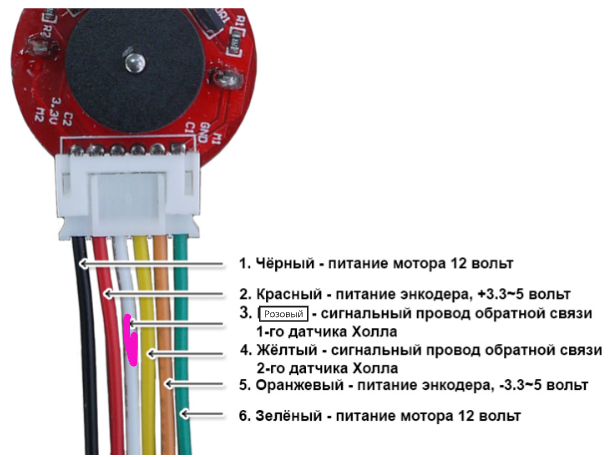
\includegraphics[width=0.95\linewidth]{./graphics/img/encoder_pinout.png}
    \caption{Распиновка энкодеров}
    \label{f:enc_pinout}
\end{figure}

При подключении двигателя нет разницы, где плюс, а где минус, поэтому предлагаю подбирать нужный результат в процессе написания кода.

Также важно сказать, что двигатели и энкодеры подключаются через аналоговые пины и управление происходит просто подачей напряжения на соответствующие выходы без всяких библиотек. Для снижения нагрузки на линии питания микроконтроллера используется драйвер.

Ниже приведён отрывок кода, который выключает моторы. Судя по моим наблюдениям, у моторов в данной конструкции робота есть всего 3 состояния: вперёд, назад и выключены. Чтобы поменять направление движения, надо поменять у всех пинов IN на OUT и наоборот.

{\ttfamily
\begin{verbatim}
    from machine import Pin


    pin_l1 = Pin(2, Pin.IN)
    pin_l2 = Pin(15, Pin.OUT)
    pin_r1 = Pin(4, Pin.IN)
    pin_r2 = Pin(0, Pin.OUT)

    pin_l2.value(0)
    pin_r2.value(0)
\end{verbatim}
}

\chapter{Ультразвуковые датчики}
Для ориентирования в пространстве в роботе "Жук" установлены шесть ультразвуковых датчиков hrc sr04. Каждый их них рассчитан на напряжение 5v, но способен работать от линии 3.3v. Питание идёт через МК, поэтому одновременное подключение всех датчиков перегружает esp32, вызывают перегрев линий питания и мешают прошивке.

В будущем необходимо расширить данный раздел информацией о библиотеке для данных датчиков, их распиновке и максимальном количестве, которое может работать от еспшки одновременно.

\chapter{Гироскоп}
Из-за проблемы с УЗ датчиками, я стал работать с гироскопом.

Результатом моей работы стал приведённый ниже код.

{\ttfamily
\begin{verbatim}
    from machine import Pin
    import utime
    from mpu6050 import mpu6050


    mpu = mpu6050.MPU6050(Pin(21, Pin.IN),
                        Pin(22, Pin.IN))

    # Функция для чтения данных с модуля MPU-6050
    def gyro_read():
        # Чтение данных акселерометра
        acc_x = mpu.get_accel_x()
        acc_y = mpu.get_accel_y()
        acc_z = mpu.get_accel_z()

        # Чтение данных гироскопа
        gyro_x = mpu.get_gyro_x()
        gyro_y = mpu.get_gyro_y()
        gyro_z = mpu.get_gyro_z()

        return acc_x, acc_y, acc_z, gyro_x, gyro_y, gyro_z

    # Основная программа
    while True:
        # Чтение данных с модуля MPU-6050
        acc_x, acc_y, acc_z, gyro_x, gyro_y, gyro_z = read_data()

        # Рассчет положения и ориентации
        roll = (acc_x + acc_y + acc_z) / 3
        pitch = (gyro_x + gyro_y + gyro_z) / 3

        # Вывод результатов
        print(f"Roll: {roll:.2f}°, Pitch: {pitch:.2f}°")

        # Ожидание следующего цикла
        utime.sleep(0.1)
\end{verbatim}
}

В теории он должен рассчитывать вращение по вертикальной оси (roll) и горизотальной (pitch), но на практике я не смог его проверить из-за особенностей программного обеспечения. По неизвестным причинам Thonny не видел библиотеку ctypes. Как один из вариантов решения этой проблемы --- включение в исполняемый файл библиотеки mpu6050 необходимых функций из зависимых пакетов, но данный подход требует глубокого знания использованных библиотек и осуществить его в рамках практики не представилось возможным.

\chapter{Подготовка отчёта}
Важной частью практики я считаю подготовку отчёта, в процессе которой я расширил свои знания о языке программирования для автоматической вёрстки документов \LaTeX{} и подготовил шаблоны для быстрого оформления будущих отчётов. В процессе я прочитал большой объём литературы, описывающей различные нюансы написания программ.

Также для оформления были изучены и учтены ГОСТы 2.105 и 7.32.


\chapter*{Заключение}
%% заключение

%\begin{thebibliography}{99}
    \bibitem{microPy}
        Официальный сайт с документацией
\end{thebibliography}

\appendix   % Тут идут приложения

%\chapter{Процедуры и схемы сбора установок и стендов}
\label{cha:appendix_schemes}

\section{Стенд для проверки точности синхронизации маяков}
\label{sec:000_sync_scheme}

\begin{enumerate}
\item Схема стенда для проверки точности синхронизации приведена на рис.~\ref{fig:000_sync_scheme}.
%\begin{figure}[ht]
%  \centering
%  \includegraphics[width=0.95\textwidth]{inc/svg/000_sync/scheme}
%  \caption{Схема стенда для проверки точности синхронизации маяков}
%  \label{fig:000_sync_scheme}
%\end{figure}


%%% Local Variables: 
%%% mode: latex
%%% TeX-master: "rpz"
%%% End: 


%\include{91-appendix2}

\end{document}

%%% Local Variables:
%%% mode: latex
%%% TeX-master: t
%%% End:
